\documentclass{article}

\usepackage{jacksonmath}
\usepackage[english]{babel}
\usepackage[utf8]{inputenc}
\usepackage[final]{pdfpages}

\begin{document}
  \section*{7.9 Problems: 1,2,3,4,8,9,19}
  \begin{enumerate}
    \item
      $\arg(1+i)=\pi/4$\\
      $\arg(1/2+\sqrt(3)/2)=1.047$\\
      $\arg((1+i)^3)=3\arg(1+i)=3\pi/4$\\
      $\arg((1/2+\sqrt(3)/2)^243)=243\arg(1/2+\sqrt(3)/2)=254.42$\\
      $\arg((1+i)^2(1/2+\sqrt(3)/2)^3)=2\arg(1+i)3\arg(1/2+\sqrt(3)/2)=2*\pi/4*3*1.047=4.934$
    \item
      \begin{enumerate}[label=(\roman*)]
        \item
          If we can make the argument continuous in this range we can simplify the expression. We can write the limit instead as $\lim_{y\to0^+}\arg(x+iy)$. We have $y>0$ so we can work in the complex plane $\C_{y>0}$ with this restriction. The function $\cos^{-1}:(-1,1)\to(0,\pi)$ is continuous on this domain.
          \begin{align*}
            \lim_{y\to0^+}\cos^{-1}\left(\frac{x}{\sqrt{x^2+y^2}}\right)&=\lim_{y\to0^+}\cos^{-1}\left(\frac{x}{\sqrt{x^2}}\right)\\
            &=\lim_{y\to0^+}\cos^{-1}\left(\frac{x}{|x|}\right)\\
            &=\lim_{y\to0^+}\cos^{-1}(-1)
          \end{align*}
          As $x/|x|\to-1$ the function $\cos^{-1}(x/|x|)\to\pi$ because it is continous.
        \item
          We can write the limit as $\lim_{y\to0^+}\arg(x-iy)$. With $y<0$ we can work in the domain $\C_{y<0}$. In this plane this function is continous:
          \[\cos^{-1}:(-1,1)\to(-\pi,0)\]
          So we can find the limit:
          \begin{align*}
            \lim_{y\to0^+}\cos^{-1}\left(\frac{x}{\sqrt{x^2+y^2}}\right)&=\lim_{y\to0^+}\cos^{-1}\left(\frac{x}{\sqrt{x^2}}\right)\\
            &=\lim_{y\to0^+}\cos^{-1}\left(\frac{x}{|x|}\right)\\
            &=\lim_{y\to0^+}\cos^{-1}(-1)
          \end{align*}
          As $x/|x|\to-1$ the function $\cos^{-1}(x/|x|)\to-\pi$ because it is continous.
      \end{enumerate}
    \item
      \begin{align*}
        &\log(3i)=\log(3)+i\pi/2\\
        &\log(-2i)=\log(2)+i3\pi/2\\
        &\log(1+i)=\log(\sqrt(2))+i\pi/4\\
        &\log(-1)=i\pi\\
        &\log((e^{i\pi/3})^{10})=10(\log|e^{i\pi/3}|+i\pi/3)=10i\pi/3\\
        &\log(x)=\begin{cases}
          x,&\text{ if }0<x\\
          \log(-x)+i\pi,&\text{ if }0>x
        \end{cases}\\
      \end{align*}
    \item
      \begin{align*}
        \Log(z_1z_2)&=\log|z_1z_2|+i\arg(z_1z_2)\\
        &=\log|z_1|+i\arg(z_1)+2iq\pi+\log|z_2|+i\arg(z_2)+2ip\pi\\
        &=\Log(z_1)+\Log(z_2)+2(q+p)i\pi
      \end{align*}
      We can let q+p=n to satisfy the equation. n can be any integer.
      \begin{align*}
        \Log(z_1)+\Log(z_2)+2i(q+r)\pi&=\Log(z_1)+2qi\pi+\Log(z_2)+2ip\pi\\
        &=\log(z_1)+\log(z_2)
      \end{align*}
    \item[8]
      \begin{enumerate}[label=(\roman*)]
        \item
          Let's find all values of n such that $(re^{i\theta})^n=1$. suppose that $r=e^a$
          \begin{align*}
            \log(1)&=\log(re^{in\theta})\\
            2im\pi&=\log(r)+in\theta+2ip\pi\\
            2im\pi-2ip\pi&=0+in\theta\\
            2\pi(m-p)/n&=\theta
          \end{align*}
          So it will the $n$th root of unity if $\theta=\frac{2im\pi}{n}$
        \item
          First we will consider $n=2$.
          \begin{align*}
            &\theta=2im\pi/2\\
            &\implies \cos(m\pi)+i\sin(m\pi)\\
            &\implies (-1)^{m}
          \end{align*}
          Next $n=3$.
          \begin{align*}
            &\theta=2im\pi/3\\
            &\implies \cos(2m\pi/3)+i\sin(2m\pi/3)\\
          \end{align*}
          So we have $(-.5-0.866i), (-0.5+0.866i), (1)$
          Finally $n=4$
          \begin{align*}
            &\theta=2im\pi/4=im\pi/2\\
            &\implies \cos(m\pi/2)+i\sin(m\pi/2)\\
          \end{align*}
          This gives us $1,i,-1,-i$
        \item
          Suppose that $\omega_1,\omega_2$ are the $n$th roots of unity.
          \begin{align*}
            ((\omega_1)^m)^n=((\omega_1)^n)^m=1^m=1\\
            (\omega_1\cdot\omega_2)^n=\omega_1^n\cdot\omega_2^n=1\\
            \left(\frac{\omega_1}{\omega_2}\right)^n=\frac{\omega_1^n}{\omega_2^n}=1
          \end{align*}
        \item
          Let's suppose that $z=de^{i\phi}$
          \begin{align*}
            z^n&=re^{i\theta}\\
            d^ne^{in\phi}&=re^{i\theta}\\
            \log(d^n)+in\phi+2im\pi&=\log(r)+i\theta+2ip\pi\\
            n\log(d)+in\phi&=\log(r)+i\theta+2i(p-m)\pi\\
            \log(d)+i\phi&=(\log(r)+i\theta+2i(p-m)\pi)/n\\
            z&=re^{i(\theta+2\pi(p-m))/n}
          \end{align*}
        \item
          Assume that $z_1^n=z_2^n$.
          \begin{align*}
            \log(z_1^n)&=\log(z_2^n)\\
            \log(z_1^n)&=\log(z_2^n)\\
            n\log|z_1|+in\arg(z_1)+2im\pi&=n\log|z_1|+in\arg(z_2)+2ip\pi\\
            \log|z_1|+i\arg(z_1)&=\log|z_2|+i\arg(z_2)+2i(p-m)\pi/n\\
            z_1=z_2e^{2i(p-m)\pi/n}
          \end{align*}
          $e^{2i(p-m)\pi/n}$ is the $n$th root of unity.
      \end{enumerate}
    \item[9]
      \begin{align*}
        1^{\sqrt{2}}&=e^{\log(1^{\sqrt{2}})}\\
        &=e^{\sqrt{2}\log(1)}=1\\
        (-2)^{\sqrt{2}}&=e^{\sqrt{2}\log(-2)}\\
        &=e^{\sqrt{2}\log(2)}e^{i\sqrt{2}\pi)}\\
        &=e^{\sqrt{2}\log(2)}(\cos(\sqrt{2}\pi)+i\sin(\sqrt{2}\pi))\\
        i^i&=e^{i\log(i)}\\
        &=e^{i(\log|i|+i\arg(i))}\\
        &=e^{-\pi/2}\\
        2^i&=e^{\log(2^i)}\\
        &=e^{i\log(2)}\\
        &=\cos(\log(2))+i\sin(\log(2))\\
        (3-4i)^{1+i}&=e^{(1+i)(\log(5)+i\arg(3-4i))}\\
        &=e^{\log(5)-\arg(3-4i)+i\arg(3-4i)+i\log(5)}\\
        &=e^{\log(5)-\arg(3-4i)}(\cos(\arg(3-4i)+\log(5))+i\sin(\arg(3-4i)+\log(5)))\\
        (3+4i)^5&=e^{5(\log(5)+i\arg(3+4i))}\\
        &=e^{5\log(5)}(\cos(\arg(3+4i))+i\sin(\arg(3+4i)))
      \end{align*}
    \item[19]
      \begin{enumerate}[label=(\roman*)]
        \item
          The choice of argument will be $\theta(t)=-t$. Thus the winding number is
          \[\frac{\theta(4\pi)-\theta(0)}{2\pi}=-2\]
          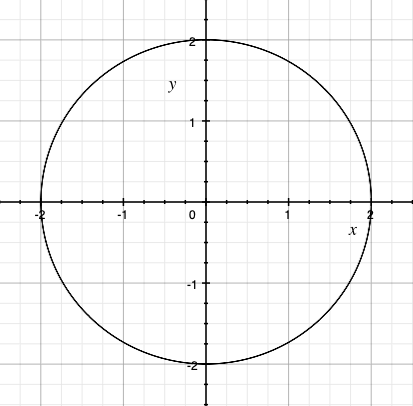
\includegraphics[scale=0.5]{g1.png}
        \item
          We will use
          \[\cos^{-1}\left(\frac{t}{\sqrt{t^{2}+\left(1-t\right)^{2}}}\right)\]
          as the the continous choice of argument. Then we get the winding number
          \[\frac{\cos^{-1}(0)-\cos^{-1}(1)}{2\pi}=1/4\]
          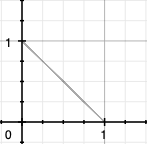
\includegraphics[scale=0.5]{g2.png}
        \item
          The choice of argument will be
          \[\cos^{-1}\left(\frac{t-1}{\sqrt{\left(t-1\right)^{2}+t^{4}}}\right)\]
          So we get the winding number:
          \[\frac{\cos^{-1}\left(-2/\sqrt{5}\right)-\cos^{-1}(0)}{2\pi}=\frac{2.67794504459-1.5707963267}{2\pi}=.176\]
          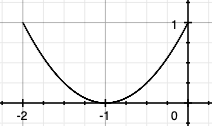
\includegraphics[scale=0.5]{g3.png}
        \item
          The continous choice of argument will be
          \[\begin{cases}
            \cos^{-1}\left(\frac{t}{\sqrt{t^{2}+(1-t)^{2}}}\right),&\text{ if }t\in[0,1]\\
            \cos^{-1}\left(\frac{1}{\sqrt{1+(t-1)^{2}}}\right),&\text{ if }t\in[1,2]
          \end{cases}\]
          So we end up with the winding number
          \[\frac{\pi/2-\pi/4}{2\pi}=1/8\]
          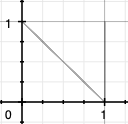
\includegraphics[scale=0.5]{g4.png}
      \end{enumerate}
  \end{enumerate}
\end{document}
